\documentclass[journal]{IEEEtran}
% Revised manuscript.  All numerical results are generated by the code in
% ../scripts and imported from numbers.tex (see export_numbers.py), so every
% value in the text can be traced to an output file.
\usepackage[utf8]{inputenc}
\usepackage[T1]{fontenc}
\usepackage{cite}
\usepackage{amsmath,amssymb,amsfonts}
\usepackage{graphicx}
\usepackage{xcolor}
\usepackage{booktabs}
\usepackage{bm}
\usepackage{siunitx}
\usepackage{tikz}
\usetikzlibrary{arrows.meta,positioning,calc,fit,backgrounds,patterns,decorations.pathmorphing}
\usepackage[hidelinks]{hyperref}
\usepackage{amsthm}
\newtheorem{proposition}{Proposition}
\newcommand{\todo}[1]{\textcolor{red}{[#1]}}
% generated by scripts/export_numbers.py -- do not edit
\newcommand{\Kmin}{21.5}
\newcommand{\Kmax}{3459}
\newcommand{\Kratio}{161}
\newcommand{\KvsamMax}{3893}
\newcommand{\FEerrMaxPct}{0.13}
\newcommand{\feA}{305.2}
\newcommand{\feB}{304.6}
\newcommand{\feC}{304.5}
\newcommand{\feD}{304.5}
\newcommand{\taucapSoft}{18.4}
\newcommand{\qdmaxSoft}{54}
\newcommand{\nlCapDropPct}{8}
\newcommand{\nlErrStiffPct}{0.7}
\newcommand{\nlErrSoftPct}{13}
\newcommand{\tmod}{1.15}
\newcommand{\modrate}{2977}
\newcommand{\Eeq}{0.031}
\newcommand{\Eload}{1.06}
\newcommand{\qdLoadDeg}{1.15}
\newcommand{\tauMone}{100}
\newcommand{\reachOrig}{2.4}
\newcommand{\feasOrigPct}{75}
\newcommand{\maxTauOrig}{160}
\newcommand{\reachStudy}{1.25}
\newcommand{\feasStudyPct}{95}
\newcommand{\maxTauStudy}{116}
\newcommand{\softOkStudyPct}{5}
\newcommand{\ikSuccPct}{96}
\newcommand{\ikItMed}{32}
\newcommand{\ikTimeA}{67}
\newcommand{\ikTimeFD}{149}
\newcommand{\ikSpeedup}{2.2}
\newcommand{\chestSoft}{0.61}
\newcommand{\chestStiff}{0.59}
\newcommand{\chestRigid}{0.51}
\newcommand{\chestGainPct}{16}
\newcommand{\handClampSoft}{0.31}
\newcommand{\handClampStiff}{0.18}
\newcommand{\handClampRigid}{0.07}
\newcommand{\armClampSoft}{0.49}
\newcommand{\armClampStiff}{0.22}
\newcommand{\mlRep}{10.7}
\newcommand{\mmRep}{7.8}
\newcommand{\isoTSchest}{0.62}
\newcommand{\secondaryMax}{41}
\newcommand{\lookupUnder}{0}
\newcommand{\lookupOverMed}{3.2}
\newcommand{\nInfeasible}{5}
\newcommand{\varSucc}{88}
\newcommand{\rigidSucc}{88}
\newcommand{\softSucc}{0}
\newcommand{\rigidRobotSucc}{88}
\newcommand{\ctRatioVarStiff}{1.00}
\newcommand{\nPairedVar}{127}
\newcommand{\utilVSSEA}{0.26}
\newcommand{\utilRigid}{0.26}
\newcommand{\utilRatioRR}{--}
\newcommand{\nSoftened}{1}
\newcommand{\softTorquePct}{100}
\newcommand{\nBound}{7}
\newcommand{\boundGainMed}{3}
\newcommand{\boundGainMax}{31}
\newcommand{\nSchedFaster}{1}
\newcommand{\schedGainMax}{14}
\newcommand{\tThreeSolved}{27}
\newcommand{\tThreeN}{45}
\newcommand{\tThreeUnsolved}{18}
\newcommand{\tThreeFailGeom}{16}
\newcommand{\refusedOK}{100}
\newcommand{\planningSummary}{The rigid-joint robot and the fixed-stiff and scheduled VSSEA planners solved the same cells: all cells of tiers~1 and~2 and \tThreeSolved\ of the \tThreeN\ feasible tier-3 cells. They also refused all \nInfeasible\ infeasible cells. Of the \tThreeUnsolved\ unsolved tier-3 cells, \tThreeFailGeom\ failed on geometry (collisions with the operator's hands or arms, or the head keep-out) that the template-based repair could not resolve; these are the cells where a stronger planner, such as an LLM using the quantitative feedback, can add value. Fixed minimum stiffness solved no cell: a torque violation appeared in the first plan of \softTorquePct\% of the feasible cells and could not be removed without stiffening. Contact limits bound the speed in \nBound\ tier-3 cells. There, the elastic arm was faster than the rigid-joint robot by a median of \boundGainMed\% (up to \boundGainMax\%), because its higher admissible speeds near the operator could be used. Everywhere else the joint-speed limit of $\pi/2$~rad/s, not safety, set the cycle time, and the cycles were identical. Stiffness scheduling shortened the cycle in \nSchedFaster\ cell (by \schedGainMax\%): with modulation costing about \tmod~s, softening rarely pays at this actuator speed.}
\newcommand{\nFaultPlans}{45}
\newcommand{\nFaultsReal}{229}
\newcommand{\fullRecall}{100.0}
\newcommand{\kinRecall}{78.6}
\newcommand{\kincRecall}{78.6}
\newcommand{\noContactRecall}{98.3}
\newcommand{\fullAgreePct}{100.0}
\newcommand{\fullFalseAlarm}{0}
\newcommand{\verifyTimeMed}{2.6}
\newcommand{\timeKinTen}{1.2}
\newcommand{\timeKinCert}{1.8}
\newcommand{\faultSummary}{The full verifier agreed with the dense reference on \fullAgreePct\% of the faulty plans and flagged \fullRecall\% of the real faults, with \fullFalseAlarm\ alarms the reference did not raise. A kinematics-only twin of the kind used in the original manuscript caught \kinRecall\% (\kincRecall\% with certified sampling). Removing the contact check lowered recall to \noContactRecall\%. The median verification time was \verifyTimeMed~s per plan.}
\newcommand{\nPost}{45}
\newcommand{\nPostReal}{36}
\newcommand{\postTen}{100}
\newcommand{\postFifty}{100}
\newcommand{\postCert}{100}
\newcommand{\postCertFA}{0}


\begin{document}

\title{Stiffness-Aware Digital-Twin Verification of LLM-Generated Plans for Collaborative Robots with Variable-Stiffness Series Elastic Actuators}

\author{Pham Van-Huy, Vu H. Trinh, Dung Tuan Ho, Thinh P. Nguyen, Than Le, Nguyen Ho Quang, and Trung Van Nguyen$^{*}$
\thanks{P. Van-Huy is with the Faculty of Information Technology, Ton Duc Thang University, Ho Chi Minh City, Vietnam (e-mail: phamvanhuy@tdtu.edu.vn).}
\thanks{V. H. Trinh, T. Le and N. H. Quang are with Thu Dau Mot University, Vietnam (e-mail: \{trinhhoaivu, ledinhthan, nguyenhoquang\}@tdmu.edu.vn).}
\thanks{D. T. Ho is with the Department of Computer Science, New Mexico State University, Las Cruces, NM, USA (e-mail: dungho@nmsu.edu).}
\thanks{T. P. Nguyen is with Wisdom Research, Ho Chi Minh City, Vietnam (e-mail: nguyenphucthinh@wisdombrain.org).}
\thanks{$^{*}$T. V. Nguyen (corresponding author) is with the Faculty of Information Technology, Van Lang School of Technology, Van Lang University, Ho Chi Minh City, Vietnam (e-mail: trung.nv@vlu.edu.vn).}}

\maketitle

\begin{abstract}
Large language models (LLMs) can turn an operator's instruction into a robot program, but the program is only useful if it respects the physics of the robot and the safety of the people next to it. For robots driven by variable-stiffness series elastic actuators (VSSEAs), the joint stiffness chosen by a planner changes how much torque a joint can carry, how far the arm deflects, and how hard the arm hits a person. We present a digital-twin verifier that models these couplings and returns quantitative repair bounds to the planner. It combines three models. The first is a leaf-spring VSSEA model, cross-checked against a plane-stress finite-element model (agreement within \FEerrMaxPct\%) and a geometrically exact beam model; it bounds the stiffness at \Kmin--\Kmax~Nm/rad and shows that the stress-limited torque capacity drops to \taucapSoft~Nm in the softest setting. The second is a contact model that maps joint stiffness to ISO/TS~15066 speed limits for free impacts, including secondary impacts, and for clamping. The third is certified collision checking on the deflected arm. For free impacts the admissible speed barely changes across the actuator's range (chest: \chestSoft\ vs.\ \chestStiff~m/s), although it is \chestGainPct\% higher than for a rigid joint; for clamping, stiffness matters strongly (hand: \handClampSoft\ vs.\ \handClampStiff~m/s, and \handClampRigid~m/s for a rigid joint). In fault-injection tests the verifier detected \fullRecall\% of real violations, against \kinRecall\% for a kinematics-only digital twin. On 150 simulated human--robot cells, verifier-guided planning solved \varSucc\% of the feasible cells, whereas fixed minimum stiffness solved \softSucc\%. Where the contact limits bound the speed (\nBound\ of \tThreeN\ demanding cells), the elastic arm was up to \boundGainMax\% faster than a rigid-joint arm; elsewhere the actuator's speed limit set the cycle time, and stiffness scheduling shortened only \nSchedFaster\ cycle. The benchmark, verifier and a pre-registered LLM evaluation protocol are released.
\end{abstract}

\begin{IEEEkeywords}
Variable stiffness actuator, series elastic actuator, digital twin, large language models, ISO/TS 15066, human--robot collaboration, verification.
\end{IEEEkeywords}

%=====================================================================
\section{Introduction}
\IEEEPARstart{C}{ollaborative} robots share their workspace with people, and safety standards such as ISO/TS~15066 \cite{iso15066} bound the force a robot may exert on each body region. Compliant actuation helps: series elastic actuators (SEAs) \cite{pratt1995} decouple the motor inertia from the link and make the joint torque measurable, and variable stiffness actuators (VSAs) \cite{vanderborght2013,wolf2016,grioli2015} let a controller trade softness against bandwidth and precision \cite{bicchi2004,albu2008}. Leaf-spring mechanisms whose effective length is changed by a roller carriage are an attractive VSA family because the stiffness can be changed with almost no energy at equilibrium and the output motion is unrestricted \cite{choi2011,sariyildiz2023,sariyildiz2024}.

At the same time, LLMs are being used to translate natural-language instructions into robot programs \cite{ahn2022,liang2023,singh2023,vemprala2023}, including in manufacturing \cite{dong2025,antero2024,yang2024autoplc} and in combination with digital twins (DTs) \cite{deng2025}. LLM outputs are not guaranteed to be physically feasible, so recent systems close the loop with an external checker \cite{skreta2023,chen2024autotamp,yang2024safety,kambhampati2024}. The checkers used so far verify geometry, joint limits or logical constraints. They do not model the actuator, so they cannot tell whether a joint can carry the payload at the stiffness the plan requests, whether the arm will sag into an obstacle, or whether an approach speed is safe for the stiffness used.

For a VSSEA-driven arm these questions cannot be separated, because the joint stiffness affects all of them at once:
\begin{itemize}
\item \emph{torque}: the leaf springs are stress-limited, so a soft setting carries less torque (here \taucapSoft~Nm in the softest setting, against the \tauMone~Nm motor limit);
\item \emph{precision}: deflection grows as $\tau/K$;
\item \emph{contact safety}: the impact and clamping forces on a person depend on the effective mass and stiffness seen at the contact point \cite{haddadin2009}.
\end{itemize}
A planner, human or LLM, therefore has to choose stiffness and speed together with the path, and a verifier has to check all three effects.

This paper builds and evaluates such a verifier. The VSSEA mechanism we model is the leaf-spring design of Sariyildiz \emph{et al.} \cite{sariyildiz2023}; we do not claim the mechanism as new. Our contributions are:
\begin{enumerate}
\item A \emph{verified actuator model chain} for the leaf-spring VSSEA: Euler--Bernoulli and Timoshenko stiffness, an independent plane-stress finite-element (FE) model, and a geometrically exact (elastica) model. The chain yields a bounded stiffness range that includes the harmonic-drive compliance, a stress-limited torque capacity as a function of stiffness, and the time and energy of stiffness modulation (Sec.~\ref{sec:vssea}).
\item A \emph{stiffness-dependent contact-safety model} that maps joint stiffness to ISO/TS~15066 speed limits. It covers free (transient) impacts, including the secondary impacts produced by the elastic transmission, and constrained (clamping) contacts. It yields a finding with design consequences: in the VSSEA range, stiffness barely changes the free-impact limit but strongly changes the clamping limit (Sec.~\ref{sec:contact}).
\item A \emph{certified, stiffness-aware digital-twin verifier}. It checks collisions on the deflected link-side configuration with a conservative-advancement guarantee, together with stress-limited torque, grasp precision and ISO/TS~15066 contact limits. It returns each violation with its magnitude and a repair bound that a planner can act on (Sec.~\ref{sec:verifier}).
\item An \emph{evaluation} comprising a 150-cell human--robot pick-and-place and hand-over benchmark; fault injection against a dense brute-force reference; a comparison of a rigid-joint robot with fixed-stiff, fixed-soft and scheduled VSSEA planners; and a pre-registered LLM protocol with feedback ablations (Sec.~\ref{sec:exp}). Code and data are released.
\end{enumerate}
The study is simulation-based: all actuator and arm parameters are design values of a virtual prototype (Table~\ref{tab:params}). Sec.~\ref{sec:discussion} discusses what a hardware study must add.

%=====================================================================
\section{Related Work}
\subsection{Compliant and variable-stiffness actuation}
SEAs \cite{pratt1995} place an elastic element between gearbox and link, which provides impact tolerance and torque sensing \cite{vanham2009}. VSAs make the stiffness adjustable; reviews classify the principles (antagonistic springs, variable pretension, variable transmission ratio, and variable spring length) and discuss their energy cost \cite{vanderborght2013,wolf2016} and their use from a control point of view \cite{grioli2015}. Bicchi and Tonietti argued that a stiffness that varies along a motion can reconcile safety and performance \cite{bicchi2004,tonietti2005}. Haddadin \emph{et al.} showed with crash tests and simulations that, at the speeds typical of service robots, the safety gain of joint elasticity comes mainly from decoupling the rotor inertia, and that further softening brings limited benefit for blunt impacts \cite{haddadin2009}. Our results for free impacts agree with this; for clamping contacts we find that stiffness matters a great deal. Leaf-spring VSAs change the effective spring length with a sliding support \cite{choi2011}. Sariyildiz \emph{et al.} built a modular VSSEA of this type with eight leaf springs and a ball-screw roller carriage, reporting a stiffness range of about \SIrange{20}{1000}{Nm/rad} and fast, low-energy modulation \cite{sariyildiz2023,sariyildiz2024}. We adopt this mechanism and add a stress-limited capacity model, an FE/elastica verification and the safety coupling needed for planning.

\subsection{Safety limits for collaborative robots}
ISO/TS~15066 \cite{iso15066} gives body-region force limits and a two-body energy model for transient contact; ISO~10218-2 \cite{iso10218_2} covers the application level. The standard's effective-mass formula is a coarse approximation, and different interpretations change the admissible speed considerably \cite{kirschner2022}. Configuration-dependent effective masses follow from the operational-space inertia \cite{khatib1987}. Villani \emph{et al.} survey safety and interfaces in industrial collaboration \cite{villani2018}. Collision detection and reaction for elastic-joint arms are described in \cite{deluca2006}; we use a detection delay and braking model of that kind for clamping.

\subsection{LLMs for robot programming and their verification}
LLMs ground instructions in robot skills \cite{ahn2022}, write policy code \cite{liang2023,vemprala2023}, produce situated plans \cite{singh2023}, and are combined with feasibility checks in task and motion planning \cite{lin2023text2motion,chen2024autotamp}. Because LLMs do not reliably plan by themselves, the LLM-Modulo view pairs them with sound external critics \cite{kambhampati2024}. Verifier-assisted iterative prompting \cite{skreta2023}, constraint monitors \cite{yang2024safety} and self-refinement \cite{madaan2023} all feed errors back to the model. In manufacturing, LLMs generate PLC code \cite{yang2024autoplc} and robot programs \cite{antero2024,dong2025}, and LLMs have been combined with DTs for multi-robot task allocation \cite{deng2025}. DTs themselves are reviewed in \cite{tao2019}, and Malik and Brem showed their value for designing collaborative cells \cite{malik2021}. None of these verifiers models the actuator's stiffness-dependent capacity or the contact forces that result; that is the gap addressed here.

%=====================================================================
\section{Variable-Stiffness Actuator Model}\label{sec:vssea}
\begin{figure}[t]
\centering
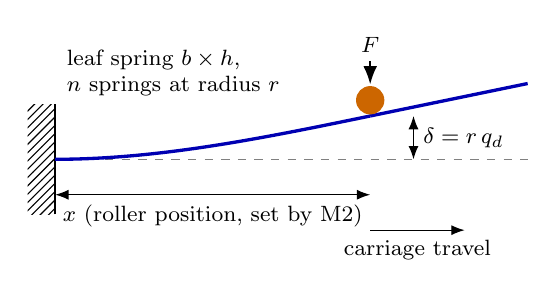
\begin{tikzpicture}[scale=1.0, every node/.style={font=\footnotesize}]
  % clamp
  \fill[pattern=north east lines] (-0.35,-0.7) rectangle (0,0.7);
  \draw[thick] (0,-0.7) -- (0,0.7);
  % undeformed spring
  \draw[gray, dashed] (0,0) -- (6,0);
  % deformed spring (cantilever shape up to roller, straight after)
  \draw[very thick, blue!70!black, domain=0:4, samples=40] plot (\x, {0.55*(3*(\x/4)^2-(\x/4)^3)/2});
  \draw[very thick, blue!70!black] (4,0.55) -- (6,{0.55+2*0.55*3/8});
  % roller
  \fill[orange!80!black] (4,0.75) circle (0.18);
  \draw[-{Latex}, thick] (4,1.25) -- (4,0.95) node[above=8pt] {$F$};
  % dimension x
  \draw[{Latex}-{Latex}] (0,-0.45) -- node[below] {$x$ (roller position, set by M2)} (4,-0.45);
  \draw[{Latex}-{Latex}] (4.55,0) -- node[right] {$\delta=r\,q_d$} (4.55,0.55);
  \draw[-{Latex}] (4,-0.9) -- node[below] {carriage travel} (5.2,-0.9);
  \node[align=left] at (1.5,1.1) {leaf spring $b\times h$,\\ $n$ springs at radius $r$};
\end{tikzpicture}
\caption{Variable-length leaf spring of the VSAM (after \cite{sariyildiz2023}). Each spring is clamped at one end. A roller carriage, positioned by the stiffness motor M2 through a ball screw, touches the spring at distance $x$. A relative rotation $q_d$ between the M1 output and the link deflects every spring by $\delta=r q_d$ at the roller.}
\label{fig:vsam}
\end{figure}

\subsection{Mechanism and assumptions}
Each joint module consists of a rigid actuator M1 (servo motor with a 1:100 harmonic drive) that sets the equilibrium position, a variable-stiffness actuation mechanism (VSAM), and a stiffness motor M2 \cite{sariyildiz2023}. Fig.~\ref{fig:vsam} shows the VSAM: $n$ leaf springs of width $b$ and thickness $h$ are arranged axially at radius $r$ and clamped at one end, and a roller carriage driven by M2 touches every spring at axial distance $x\in[x_{\min},x_{\max}]$ from the clamp. Table~\ref{tab:params} lists the design values of our virtual prototype. They were chosen so that the stiffness span is comparable to the range published for the physical device \cite{sariyildiz2023}; they are not measurements.

\subsection{Stiffness}
Under a transverse load $F$ at the roller, an Euler--Bernoulli cantilever deflects by $\delta = Fx^3/(3EI)$ with $I=bh^3/12$. Adding Timoshenko shear compliance \cite{cowper1966} gives the transverse spring rate
\begin{equation}
k_b(x)=\left(\frac{x^3}{3EI}+\frac{x}{\kappa G b h}\right)^{-1},\qquad \kappa=5/6 .
\end{equation}
With $\delta=r q_d$ and torque $\tau=nFr$, the VSAM and joint stiffnesses are
\begin{equation}
K_\mathrm{v}(x)=n\,k_b(x)\,r^2,\qquad K(x)=\left(K_\mathrm{v}(x)^{-1}+K_\mathrm{hd}^{-1}\right)^{-1},
\label{eq:K}
\end{equation}
where $K_\mathrm{hd}$ is the torsional stiffness of the harmonic drive in series. Eq.~\eqref{eq:K} answers the claim, made for this class of mechanism, of a ``near-zero to infinite'' stiffness range. $K_\mathrm{v}$ grows as $x^{-3}$, but $x$ cannot be smaller than the roller and clamp dimensions, and the series compliance caps the joint stiffness below $K_\mathrm{hd}$. For our design $K\in[\Kmin,\Kmax]$~Nm/rad, a ratio of \Kratio.

\subsection{Stress-limited torque capacity}
The root bending stress of a spring is $\sigma=Fx(h/2)/I$. Limiting it to $\sigma_\mathrm{a}$ (yield over a safety factor of 1.6) gives the linear capacity
\begin{equation}
\tau_\mathrm{cap}^\mathrm{lin}(x)=\frac{n\,\sigma_\mathrm{a}\,b\,h^2\,r}{6\,x}.
\label{eq:cap}
\end{equation}
Because $K\propto x^{-3}$ while $\tau_\mathrm{cap}\propto x^{-1}$, a softer joint can carry less torque. At the soft end the allowable deflection is large ($q_d\approx\qdmaxSoft^\circ$), so we also solve the geometrically exact elastica of a clamped strip pushed by a frictionless roller, whose contact force is normal to the deformed beam (shooting on the contact arc length, contact angle, force and root moment). The verifier uses the smaller of the linear and elastica capacities, interpolated in $K$.

\subsection{Stiffness modulation}
At equilibrium the roller force is normal to the carriage motion, so holding or changing stiffness requires work only against rolling friction. Under a deflection $q_d$ the deformed spring has slope $\varphi\approx 3\delta/(2x)$ at the contact, which produces an axial reaction $F_\mathrm{ax}=nF\varphi$ on the carriage. M2 must work against this reaction when stiffening under load. Modulation time follows from a trapezoidal M2 speed profile through the ball-screw lead.

\subsection{Joint model used by the twin}
Each joint is a two-mass elastic joint \cite{spong1987}. The controller feeds forward the static spring deflection $\tau_g/K$ (gravity compensation for elastic joints \cite{deluca2005}). The twin therefore applies a residual fraction $\rho$ of the static deflection, representing stiffness and payload model error, plus the uncompensated inertial deflection:
\begin{equation}
\bm q_\ell=\bm q_c-\bm K^{-1}\left(\rho\,\bm\tau_g(\bm q_\ell)+\bm M(\bm q_\ell)\ddot{\bm q}_c\right),
\label{eq:defl}
\end{equation}
which is solved by fixed-point iteration. The joint torque that must stay below $\min(\tau_{M1},\tau_\mathrm{cap}(K))$ is the full $\bm\tau_g+\bm M\ddot{\bm q}_c$.

%=====================================================================
\section{Arm Model}\label{sec:arm}
\emph{Correction to the earlier kinematics.} The earlier version of this work described the arm with nine Denavit--Hartenberg (DH) frames, all with $a_i=0$, and called it both ``6-DOF'' and ``9-link''. Taken literally, that chain stacks two \SI{0.76}{m} offsets with alternating $\pm90^\circ$ twists. It reaches \reachOrig~m, its elbow hangs below the work surface in tool-down poses, and with \tauMone~Nm actuators it can hold a \SI{2.5}{kg} payload in only \feasOrigPct\% of random configurations: joint~2 needs up to \maxTauOrig~Nm (Fig.~\ref{fig:workspace}a). The chain does not describe a collaborative arm that these actuators could drive.

\emph{Arm used in this study.} We therefore place VSSEA modules on the kinematic structure of a widely used 6-DOF collaborative arm, the UR5e, using the manufacturer's DH parameters (Table~\ref{tab:dh}) plus a \SI{0.15}{m} gripper. The mass model lumps a \SI{2.8}{kg} module at every moving joint, tube links of \SI{1.2}{kg/m} and the payload at the tool centre point (TCP). Gravity torques are checked against the gradient of the potential energy (error $<10^{-5}$~Nm). With a \SI{2.5}{kg} payload, \feasStudyPct\% of random configurations can be held; joint~2 needs up to \maxTauStudy~Nm near full extension. Only \softOkStudyPct\% can be held with all joints in the softest setting (Fig.~\ref{fig:workspace}b), so torque feasibility bounds the stiffness from below during most motions. Inverse kinematics (IK) uses damped least squares \cite{wampler1986} on position and tool axis with the analytic Jacobian. The twin resolves the IK branch as a controller would: among the solutions reached from the current configuration and from elbow-up seeds facing the target, it selects the closest one whose joint path is free of collisions on a coarse check. The certified check of Sec.~\ref{sec:verifier} then verifies the path.

\begin{table}[t]
\caption{Kinematics of the study arm (UR5e structure, standard DH; m, rad)}\label{tab:dh}
\centering\footnotesize
\begin{tabular}{ccccc}
\toprule
Joint & $a_i$ & $d_i$ & $\alpha_i$ & limits\\
\midrule
1 & 0 & 0.1625 & $\pi/2$ & $\pm2\pi$\\
2 & $-0.425$ & 0 & 0 & $\pm2\pi$\\
3 & $-0.3922$ & 0 & 0 & $\pm2\pi$\\
4 & 0 & 0.1333 & $\pi/2$ & $\pm2\pi$\\
5 & 0 & 0.0997 & $-\pi/2$ & $\pm2\pi$\\
6 & 0 & $0.0996+0.15$ (gripper) & 0 & $\pm2\pi$\\
\bottomrule
\end{tabular}
\end{table}

\begin{figure*}[t]
\centering
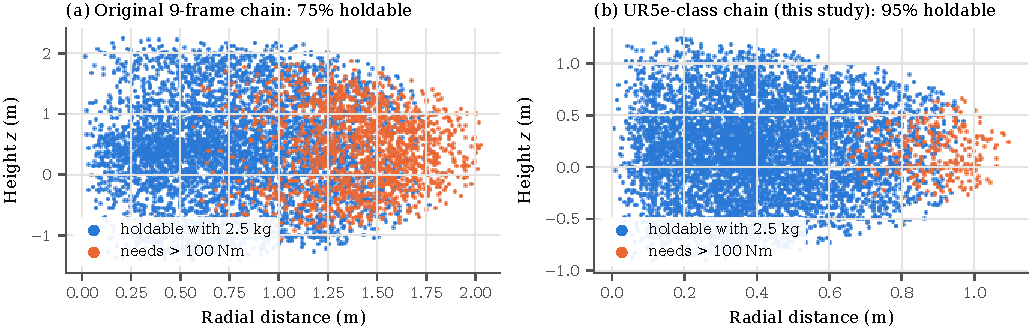
\includegraphics[width=\textwidth]{../figures/fig_workspace.pdf}
\caption{Configurations that can hold a \SI{2.5}{kg} payload with \tauMone~Nm actuators (\num{20000} random configurations). (a) Nine-frame chain of the earlier manuscript. (b) UR5e-class chain used here.}
\label{fig:workspace}
\end{figure*}

%=====================================================================
\section{Stiffness-Dependent Contact Safety}\label{sec:contact}
\subsection{Body model}
ISO/TS~15066 gives, for each body region $b$, a quasi-static force limit $F_{\mathrm{qs},b}$, a transient limit $F_{\mathrm{T},b}=2F_{\mathrm{qs},b}$ (not permitted for skull and face), an effective spring constant $k_b$ and an effective mass $m_{\mathrm{H},b}$ \cite{iso15066}. The standard's transient model treats the robot as a rigid mass $m_R$ and gives $v_{\max}=F_{\mathrm{T},b}/\sqrt{\mu k_b}$ with $\mu^{-1}=m_R^{-1}+m_{\mathrm{H},b}^{-1}$.

\subsection{Reduced impact model for an elastic joint}
For a contact at point $\bm p$ on the arm along the unit normal $\bm u$, let $\bm a=\bm J_p^\top\bm u$. We project the link-side inertia $\bm M_\ell$, the inertia with reflected rotors $\bm M_r=\bm M_\ell+N^2J_m\bm I$, and the joint compliance onto $\bm u$ \cite{khatib1987}:
\begin{equation}
m_\ell=(\bm a^\top\bm M_\ell^{-1}\bm a)^{-1},\quad m_m=(\bm a^\top\bm M_r^{-1}\bm a)^{-1}-m_\ell,\quad K_c=(\bm a^\top\bm K^{-1}\bm a)^{-1}.
\end{equation}
The contact is then modelled as the chain $m_m$--$K_c$--$m_\ell$--$k_b$--$m_{\mathrm{H},b}$ with a unilateral contact spring and 5\% transmission damping. The model is piecewise linear and positively homogeneous, so the peak force is $F_\mathrm{pk}=g\,v$ with a gain $g(m_\ell,m_m,K_c,b)$ that does not depend on the impact speed $v$. We compute $g$ exactly with mode-wise matrix exponentials and with event handling for loss and re-establishment of contact. Simulation continues until an energy bound proves that the link can no longer catch up with the body. Two limits are recovered exactly: $K_c\to\infty$ gives the rigid ISO formula with $m_R=m_\ell+m_m$, and $K_c\to0$ gives the link-only formula. Against an independent variable-step ODE solution the error is below $10^{-4}$.

Secondary impacts matter. When the motor side keeps pushing through a soft transmission, the link can strike the body again after the first contact has ended. Over 200 random torso contacts with realistic reduced masses and stiffnesses, this raised the peak force by up to \secondaryMax\% compared with a first-impact-only model, so the verifier always uses the full model.

\subsection{Clamping}
If a fixed surface lies behind the body part along $\bm u$ (within the part's radius plus \SI{10}{cm}), the contact is treated as constrained ($m_\mathrm{H}\to\infty$). After a detection delay $t_d=\SI{30}{ms}$ (collision detected from the spring torque \cite{deluca2006}) the motor side brakes at \SI{3}{m/s^2} and holds its position. The peak force over \SI{0.5}{s} must stay below $F_{\mathrm{T},b}$, and the residual clamping force $(K_c^{-1}+k_b^{-1})^{-1}s$, with motor over-travel $s=vt_d+v^2/(2a_b)$, must stay below $F_{\mathrm{qs},b}$. Here the joint stiffness enters directly.

\subsection{Lookup and conservativeness}
For speed, $g$ is tabulated on a logarithmic grid ($18\times18\times28$ per body model) and the clamping limit on a $14\times20$ grid. A query returns the worst value of its grid cell plus a 1\% margin. On 300 random queries the lookup under-estimated the force \lookupUnder\ times; it over-estimated it by \lookupOverMed\% (median).

\subsection{Results: what stiffness does to the speed limits}
\begin{figure*}[t]
\centering
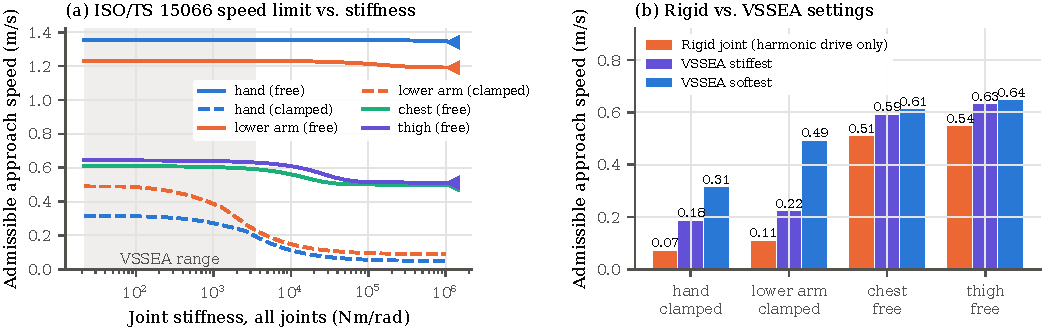
\includegraphics[width=\textwidth]{../figures/fig_contact.pdf}
\caption{(a) Admissible approach speed of the wrist module (arm reaching \SI{0.6}{m}, horizontal approach) as a function of the stiffness of all joints, for free (solid) and clamped (dashed) contacts. Triangles: ISO/TS~15066 formula with the rigid configuration-dependent mass. Shaded: VSSEA range. (b) The same limits for a rigid joint (harmonic drive only), the stiffest VSSEA setting and the softest.}
\label{fig:contact}
\end{figure*}
Fig.~\ref{fig:contact} separates the two regimes for a representative configuration: the wrist module moving horizontally with the arm reaching \SI{0.6}{m}, with link-side mass \mlRep~kg and reflected motor mass \mmRep~kg.
\begin{itemize}
\item \emph{Free impacts.} Across the actuator range the limit hardly changes (chest \chestSoft\ vs.\ \chestStiff~m/s), because every VSSEA setting already decouples most of the rotor inertia during the short contact. It is \chestGainPct\% higher than for a joint with only harmonic-drive compliance (\chestRigid~m/s).
\item \emph{Clamping.} When a hand can be pinned against the bench, the admissible speed falls from \handClampSoft~m/s (softest) to \handClampStiff~m/s (stiffest), and to \handClampRigid~m/s for the rigid joint; for the lower arm the corresponding values are \armClampSoft\ and \armClampStiff~m/s.
\end{itemize}
The standard's own formula ($m_R=M/2+m_L$) gives \isoTSchest~m/s for the chest. That exceeds the configuration-dependent rigid value, illustrating the interpretation issues discussed in \cite{kirschner2022}. Stiffness scheduling can therefore pay off near surfaces where the operator's hands may be pinned, not in open space. The planner prompt and the verifier feedback both encode this distinction.

%=====================================================================
\section{Stiffness-Aware Digital-Twin Verifier}\label{sec:verifier}
\begin{figure*}[t]
\centering
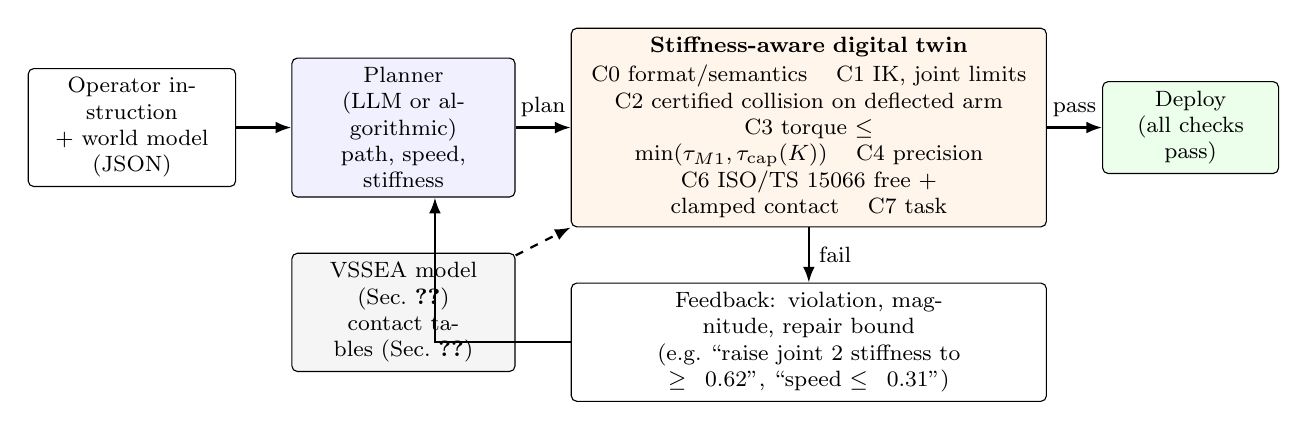
\begin{tikzpicture}[node distance=4mm and 7mm, every node/.style={font=\footnotesize},
  box/.style={draw, rounded corners=2pt, align=center, minimum height=10mm, fill=white},
  arr/.style={-{Latex[length=2mm]}, thick}]
  \node[box, text width=24mm] (op) {Operator instruction\\ + world model (JSON)};
  \node[box, text width=26mm, right=of op, fill=blue!6] (llm) {Planner\\ (LLM or algorithmic)\\ path, speed, stiffness};
  \node[box, text width=58mm, right=of llm, fill=orange!8] (dt) {\textbf{Stiffness-aware digital twin}\\[1pt]
     C0 format/semantics \;\; C1 IK, joint limits\\
     C2 certified collision on deflected arm\\
     C3 torque $\le \min(\tau_{M1},\tau_\mathrm{cap}(K))$ \;\; C4 precision\\
     C6 ISO/TS 15066 free + clamped contact \;\; C7 task};
  \node[box, text width=20mm, right=of dt, fill=green!8] (dep) {Deploy\\ (all checks pass)};
  \node[box, text width=58mm, below=7mm of dt] (fb) {Feedback: violation, magnitude, repair bound\\ (e.g.\ ``raise joint 2 stiffness to $\ge 0.62$'', ``speed $\le 0.31$'')};
  \node[box, text width=26mm, below=7mm of llm, fill=gray!8] (models) {VSSEA model (Sec.~\ref{sec:vssea})\\ contact tables (Sec.~\ref{sec:contact})};
  \draw[arr] (op) -- (llm);
  \draw[arr] (llm) -- node[above]{plan} (dt);
  \draw[arr] (dt) -- node[above]{pass} (dep);
  \draw[arr] (dt) -- node[right]{fail} (fb);
  \draw[arr] (fb.west) -| ($(llm.south)+(4mm,0)$);
  \draw[arr, dashed] (models) -- (dt.south west);
\end{tikzpicture}
\caption{Closed-loop architecture. A plan reaches the robot only after the twin has accepted it; a rejected plan is returned with quantitative feedback.}
\label{fig:arch}
\end{figure*}

\subsection{Plan representation}
A plan (Fig.~\ref{fig:arch}) is a JSON list of \texttt{move}, \texttt{grasp} and \texttt{release} steps. A \texttt{move} names a target (coordinates, an item or a location, with an optional offset), a speed fraction and a stiffness level $s\in[0,1]$, either one per joint or one shared. The level maps logarithmically to $K=K_{\min}(K_{\max}/K_{\min})^s$. The tool points down; joints interpolate linearly in joint space with a synchronized trapezoidal profile ($\dot q_{\max}=s_v\pi/2$~rad/s). A stiffness change is executed before the move and costs the M2 modulation time. A plan may instead declare the task infeasible.

\subsection{Checks}
The twin executes the plan and evaluates the following checks along the motion:
\begin{itemize}
\item C0 schema and semantics: ids, gripper state.
\item C1 reachability and joint limits.
\item C2 clearance of $\ge\SI{10}{mm}$ between the link capsules or the carried item and the obstacles, other items and the operator, plus self-collision, all on the deflected configuration \eqref{eq:defl}.
\item C3 joint torque within $\min(\tau_{M1},\tau_\mathrm{cap}(K))$.
\item C4 tool error at grasp ($\le\SI{10}{mm}$) and release height ($\le\SI{15}{mm}$).
\item C6 the ISO/TS~15066 speed limit for every robot--body pair closer than \SI{0.45}{m}, using the approach speed $\bm u^\top\bm J_p\dot{\bm q}$, and a \SI{30}{cm} keep-out around the head.
\item C7 task completion.
\end{itemize}
Each violation carries its magnitude and, where one exists, a repair bound: the minimum stiffness level for the torque, the maximum speed fraction for contact, a softer per-joint stiffness vector that raises the contact limit while staying torque-feasible, or the height correction at release.

\subsection{Certified sampling}
\begin{proposition}
Let $R_j$ bound the distance from joint axis $j$ to any point of the arm and carried item distal to it, and let $V=\eta\sum_j R_j|\dot q_j|_{\max}$ with $\eta\ge1$ covering the change of elastic deflection. If at sample $t_i$ the minimum clearance (after the safety margin) is $c_i>0$ and $t_{i+1}-t_i\le c_i/V$, then no point of the arm penetrates the margin on $[t_i,t_{i+1}]$.
\end{proposition}
\begin{proof}[Proof sketch]
The velocity of any arm point is bounded by $\sum_j R_j|\dot q_j|$, so its displacement over the interval is below $c_i$. This is conservative advancement for articulated chains \cite{schwarzer2005}.
\end{proof}
The verifier steps adaptively with $h_i=\mathrm{clip}(c_i/V,h_{\min},h_{\max})$, using exact segment--segment and segment--box distances \cite{ericson2004}. The guarantee holds for the twin's geometric model with $\eta=1.2$; we validate it empirically against dense sampling in Sec.~\ref{sec:faults}.

\subsection{Planners}
\emph{Algorithmic repair.} The planner starts from a pick-and-place template: rise to a safe height, follow an arc around the base on the side away from the operator, and descend vertically. It then applies the verifier's repair bounds:
\begin{itemize}
\item stiffen the joint named in a torque violation;
\item insert a via point after a collision;
\item scale down the speed, or apply the softer stiffness vector, after a contact violation;
\item correct the release height.
\end{itemize}
Once a plan passes, a speed pass raises every move to full speed, including the final approaches next to the operator, subject to the contact limits. The \emph{scheduled} planner additionally tries, for each block of transit moves, the minimum torque-feasible stiffness computed from the verified trajectory (30\% margin). It keeps whichever option, stiff or softened, verifies with the shorter cycle, so it can never be slower than fixed-stiff. The \emph{fixed-stiff} and \emph{fixed-soft} baselines freeze the stiffness at $s=1$ or $s=0$. The \emph{rigid-joint robot} uses the same arm with conventional joints: only harmonic-drive compliance ($K=K_\mathrm{hd}$) and full motor torque at any setting. A task is declared infeasible only if a torque violation cannot be removed at any stiffness.

\emph{LLM planner.} The LLM receives a capability sheet (stiffness levels with their torque capacities, the safety rules and the ISO body-region limits), the world model and the instruction, and returns a JSON plan. Five conditions isolate the role of feedback: \emph{zero-shot} (one attempt, as in the original manuscript); \emph{binary} feedback; \emph{qualitative} feedback (violation types only); \emph{quantitative} feedback (magnitudes and repair bounds, proposed); and \emph{quantitative with fixed stiffness} (an ablation). Each condition allows at most five rounds.

%=====================================================================
\section{Experiments}\label{sec:exp}
\begin{table}[t]
\caption{Virtual-prototype parameters}\label{tab:params}
\centering\footnotesize
\begin{tabular}{lr}
\toprule
Leaf springs $n$, $b\times h$, radius $r$ & 8, \SI{20}{mm}$\times$\SI{2}{mm}, \SI{40}{mm}\\
Spring steel $E$, $\sigma_\mathrm{a}$ & \SI{206}{GPa}, \SI{800}{MPa}\\
Roller travel $[x_{\min},x_{\max}]$ & \SIrange{30}{170}{mm}\\
Harmonic drive ratio, $K_\mathrm{hd}$ & 100, \SI{3.1e4}{Nm/rad}\\
M1 torque, joint speed & \tauMone~Nm, $\pi/2$~rad/s\\
M2: ball-screw lead, max speed & \SI{2}{mm}, \SI{4000}{rpm}\\
Module mass, link density, payload & \SI{2.8}{kg}, \SI{1.2}{kg/m}, $\le$\SI{2.5}{kg}\\
Rotor inertia $J_m$ & \SI{1.2e-4}{kg.m^2}\\
Residual static deflection $\rho$ & 0.10\\
\bottomrule
\end{tabular}
\end{table}

\subsection{Setup and benchmark}
All experiments run in Python with the released code; Table~\ref{tab:params} lists the parameters. The benchmark contains 150 procedurally generated cells: 50 per tier.
\begin{itemize}
\item Tier~1: a source and a target station, no person.
\item Tier~2: an operator at a separate assembly bench.
\item Tier~3: the operator beside the source or target, with heavier parts (\SIrange{1.2}{2.5}{kg}) and an overhead beam or a tall bin. In about half of these cells the part must be handed over onto the robot side of the operator's bench, next to the operator's hands.
\end{itemize}
Every cell also contains a distractor item. \nInfeasible\ tier-3 cells contain a part that is too heavy to lift (\SIrange{9}{14}{kg}); for these the correct output is a refusal. The operator is modelled by 15 capsules labelled with ISO body regions. Each cell has a natural-language instruction (e.g.\ ``Pick up the black motor cover from the fixture table and place it on the conveyor. An operator is working at the assembly bench.'' or, for a hand-over, ``Transfer the grey housing from the inspection bench and place it on the operator's assembly bench (hand-over). The operator is working at the assembly bench; hand the part over onto the robot side of the bench.'').

\subsection{E1: actuator model verification}
\begin{figure*}[t]
\centering
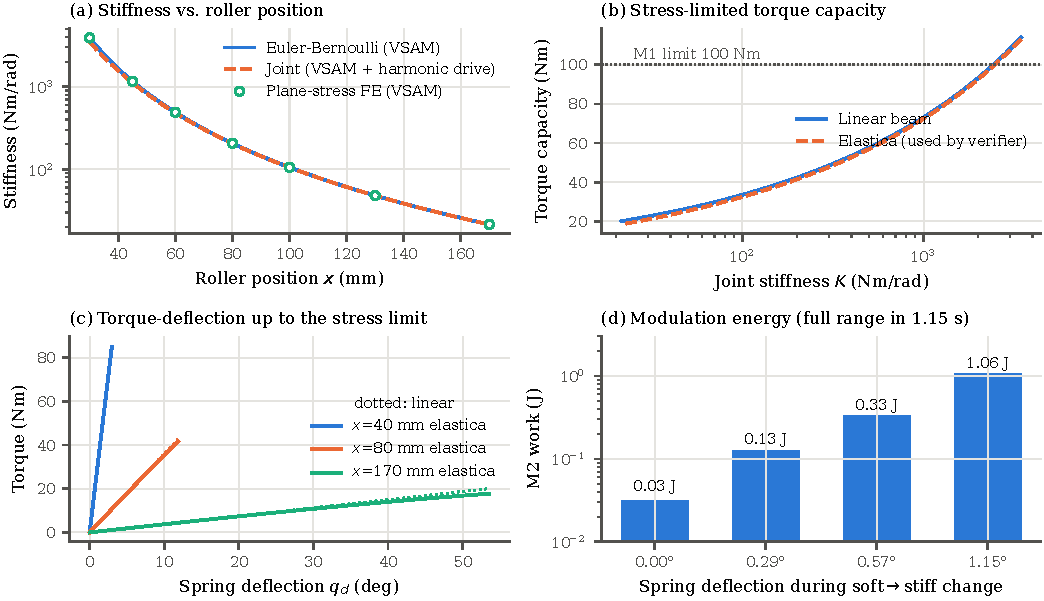
\includegraphics[width=\textwidth]{../figures/fig_vssea.pdf}
\caption{VSAM model verification. (a) Joint and VSAM stiffness: the FE results (markers) agree with beam theory within \FEerrMaxPct\%. (b) The stress-limited capacity falls with stiffness; the elastica is up to \nlCapDropPct\% below the linear model at the soft end. (c) Linear (dotted) vs.\ geometrically exact torque--deflection. (d) M2 work for a full soft-to-stiff change at different spring deflections.}
\label{fig:vssea}
\end{figure*}
Fig.~\ref{fig:vssea} summarizes the actuator model.
\begin{itemize}
\item \emph{Stiffness.} The plane-stress FE model, using quadratic 8-node elements and converged under mesh refinement (Table~\ref{tab:fe}), agrees with the Timoshenko model within \FEerrMaxPct\% over the whole roller travel. Shear compliance is negligible ($<0.4\%$ at $x_{\min}$), so Euler--Bernoulli is adequate for stiffness.
\item \emph{Upper bound.} The harmonic drive limits the joint stiffness to \Kmax~Nm/rad, while the VSAM alone would reach \KvsamMax~Nm/rad.
\item \emph{Nonlinearity.} At the stress limit, the linear model over-predicts the torque by \nlErrStiffPct\% in the stiffest setting and by \nlErrSoftPct\% in the softest; the verifier therefore uses the elastica capacity.
\item \emph{Modulation.} A full soft-to-stiff change takes \tmod~s (\modrate~Nm/rad/s). It costs \Eeq~J at equilibrium but \Eload~J when the springs are deflected by \qdLoadDeg$^\circ$, so stiffness should be changed while the joint is lightly loaded. The verifier charges this time and energy to the plan.
\end{itemize}

\begin{table}[t]
\caption{FE mesh convergence (transverse stiffness at $x=\SI{30}{mm}$)}\label{tab:fe}
\centering\footnotesize
\begin{tabular}{lcccc}
\toprule
Elements (length$\times$thickness) & 30$\times$1 & 60$\times$2 & 120$\times$4 & 240$\times$6\\
\midrule
$k_b$ (kN/m) & \feA & \feB & \feC & \feD\\
\bottomrule
\end{tabular}
\end{table}

\subsection{E2: arm model}
Over 200 random reachable tool-down targets, DLS IK converged in \ikSuccPct\% of cases (median \ikItMed\ iterations). The analytic Jacobian (\ikTimeA~ms per solve, including restarts) and the finite-difference Jacobian of the original manuscript (\ikTimeFD~ms) gave identical solutions; the analytic form is \ikSpeedup$\times$ faster. Fig.~\ref{fig:workspace} compares the torque-feasible workspaces of the two kinematic chains.

\subsection{E3: contact safety}
Reported in Sec.~\ref{sec:contact} and Fig.~\ref{fig:contact}.

\subsection{E4: verifier soundness by fault injection}\label{sec:faults}
We took \nFaultPlans\ plans accepted by the full verifier in E5 (scheduled planner, up to 15 per tier) and injected seven fault types:
\begin{itemize}
\item the first transit waypoint driven \SI{3}{cm} into the source station;
\item a \SI{6}{mm} thick, \SI{1.2}{m} wide guard plate across a transit move;
\item minimum stiffness on all loaded moves;
\item maximum speed near the operator;
\item a plan tuned for soft joints executed stiff and faster;
\item grasping the wrong item;
\item a \SI{12}{cm} placement offset.
\end{itemize}
The reference is the full model sampled densely (150 samples per move); a faulty plan counts only if the reference rejects it. Table~\ref{tab:faults} compares the checkers. \faultSummary{} Contact faults (over-speed near the operator, a soft-tuned plan executed stiff) became real violations in only two plans. This is consistent with E5: at the actuator's speed limit the ISO limits rarely bind. Both of those violations were caught only by the full verifier.

\emph{Does certified sampling matter?} To isolate the sampling scheme, we compared kinematic checkers that differ only in sampling. They were tested on a short pin ($8\times8\times40$~mm) placed on the tool path, at 15\% of the longest move of each of the \nPost\ plans of the E4 subset. The dense reference (500 samples per move) found a collision in \nPostReal\ plans. Ten fixed samples per move caught \postTen\%, fifty caught \postFifty\%, and conservative advancement caught \postCert\%, with \postCertFA\ false alarms; a taller (\SI{60}{cm}) post was likewise caught by every scheme. At the scale of these cells, coarse sampling therefore missed nothing. What conservative advancement adds is a guarantee, at a median cost of \timeKinCert~s against \timeKinTen~s per plan for the kinematic checks.

\begin{table}[t]
\caption{Detected faults (recall, \%) against the dense reference. Kin.\ 10 / Kin.\ cert.: kinematic checks only (as in the original manuscript) with 10 fixed samples per move or certified sampling; No contact: full model without the ISO/TS~15066 check; Full: proposed verifier.}\label{tab:faults}
\centering\footnotesize
\resizebox{\columnwidth}{!}{\setlength{\tabcolsep}{3pt}\begin{tabular}{lccccc}
\toprule
Fault & $n$ & Kin.\ 10 & Kin.\ cert. & No contact & Full \\
\midrule
obstacle intrusion & 45 & 100 & 100 & 100 & 100 \\
overspeed near human & 2 & 0 & 0 & 0 & 100 \\
place offset & 45 & 100 & 100 & 100 & 100 \\
rigid assumption & 2 & 0 & 0 & 0 & 100 \\
thin obstacle & 45 & 100 & 100 & 100 & 100 \\
under stiffness & 45 & 0 & 0 & 100 & 100 \\
wrong item & 45 & 100 & 100 & 100 & 100 \\
\midrule
All & 229 & 79 & 79 & 98 & 100 \\
\bottomrule
\end{tabular}}
\end{table}

\subsection{E5: planning benchmark}
\begin{figure*}[t]
\centering
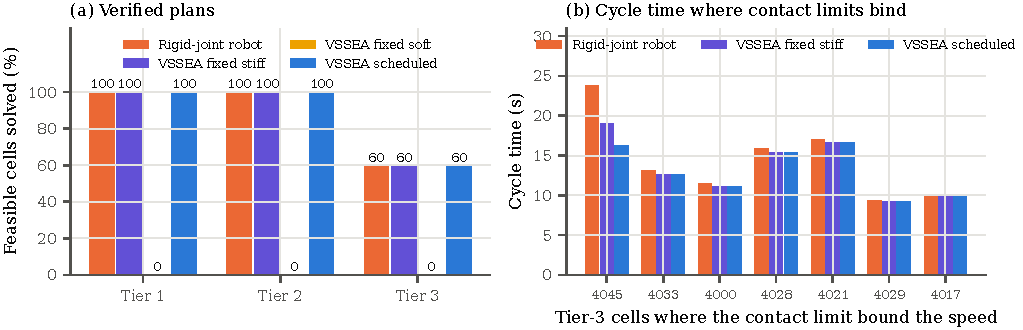
\includegraphics[width=\textwidth]{../figures/fig_planning.pdf}
\caption{Algorithmic planners on the 150-cell benchmark. (a) Share of feasible cells with a verified plan, by tier. (b) Cycle times in the tier-3 cells where a contact limit bound the speed and the elastic arm was faster than the rigid-joint robot.}
\label{fig:planning}
\end{figure*}
\begin{table}[t]
\caption{Planning benchmark (150 cells). Solved: feasible cells with a verified plan. Refusals: infeasible cells correctly declared infeasible. Cycle: median over solved cells. ISO util.: median over cells with an operator of the largest ratio of approach speed to admissible speed.}\label{tab:planning}
\centering\footnotesize
\resizebox{\columnwidth}{!}{\begin{tabular}{lccccc}
\toprule
Planner & Solved (\%) & T1 / T2 / T3 (\%) & Refusals (\%) & Cycle (s) & ISO util. \\
\midrule
Rigid-joint robot & 88 & 100 / 100 / 60 & 100 & 11.3 & 0.26 \\
VSSEA, fixed stiff & 88 & 100 / 100 / 60 & 100 & 11.3 & 0.26 \\
VSSEA, fixed soft & 0 & 0 / 0 / 0 & 0 & -- & -- \\
VSSEA, scheduled (ours) & 88 & 100 / 100 / 60 & 100 & 11.3 & 0.26 \\
\bottomrule
\end{tabular}}
\end{table}
Table~\ref{tab:planning} and Fig.~\ref{fig:planning} report the results. \planningSummary

\subsection{E6: LLM planning protocol}
The harness (\texttt{vsdt/llm}) runs the five feedback conditions on all 150 cells with three seeds per condition (temperature 0.2), for any OpenAI-compatible endpoint (including local models via Ollama or vLLM) or the Anthropic API. Success is the share of episodes that end in a verified plan, or in a refusal for an infeasible cell. We report Wilson 95\% intervals \cite{wilson1927} and exact McNemar tests \cite{mcnemar1947}, paired by cell and seed, of every condition against the quantitative condition, with Holm correction \cite{holm1979}. We also record how often the \emph{first} plan would have been unsafe if deployed without the gate. \todo{Table~\ref{tab:llm} is filled by \texttt{python -m vsdt.llm.analyze}; insert the models used and summarize the outcome here once the runs are complete.}

\begin{table}[t]
\caption{LLM planning results (95\% Wilson intervals)}\label{tab:llm}
\centering\scriptsize
\IfFileExists{llm_table.tex}{\resizebox{\columnwidth}{!}{\input{llm_table.tex}}}{\todo{run the LLM harness}}
\end{table}

%=====================================================================
\section{Discussion}\label{sec:discussion}
\emph{What the verifier guarantees.} A plan that passes is collision-free with the stated margin, torque-feasible and within the modelled ISO/TS~15066 limits, for the twin's models. ``Zero unsafe deployments'' is therefore a property of the gate, not an empirical achievement of the LLM. The empirical questions are how often the LLM reaches a verified plan, how quickly, and at what cycle time; E6 measures these. The previous version of this work reported ``100\% safety reliability''; we now state that claim precisely, in this conditional form.

\emph{Role of stiffness.} Within the VSSEA range, stiffness has little effect on free-impact limits but a large one on clamping limits, and it sets the torque that a joint can carry. A good schedule is therefore stiff where the arm carries load and where precision matters, and soft near surfaces where the operator's hands may be pinned. In our benchmark the actuator's joint-speed limit ($\pi/2$~rad/s, taken from the published prototype \cite{sariyildiz2023}) kept the arm below the ISO/TS~15066 limits almost everywhere. Softening therefore rarely repaid its modulation time of about \SI{1}{s}; scheduling shortened \nSchedFaster\ cycle. The elastic transmission itself paid off in the \nBound\ cells where contact limits bound the speed, with gains of up to \boundGainMax\% over a rigid-joint arm. Faster actuators, or tasks dominated by clamping-prone motions, are where scheduling should pay. The verifier quantifies this case by case, which is what a planner needs.

\emph{Limitations.}
\begin{itemize}
\item There is no hardware validation. The actuator parameters are design values comparable to a published prototype \cite{sariyildiz2023}, the arm uses a published kinematic structure with an assumed mass model, and the masses are estimates.
\item Joint dynamics are quasi-static plus inertial deflection. Link oscillation in soft modes is not simulated, and neither is the controller.
\item The operator is static.
\item Contact uses a one-dimensional reduced model with ISO body parameters, whose interpretation is debated \cite{kirschner2022}.
\item The clamping model assumes no retraction.
\item The benchmark is procedurally generated.
\end{itemize}
A hardware study should measure the stiffness and capacity curves, the modulation time and energy, and contact forces with a biofidelic measurement device in clamped and free settings.

\section{Conclusion}
We built a digital-twin verifier that understands what a variable-stiffness actuator can and cannot do and used it to correct LLM-generated plans for a collaborative arm. The actuator model is verified against FE and large-deflection solutions. It bounds the stiffness range and shows that torque capacity falls with stiffness. The contact model shows that the VSSEA's stiffness matters mainly for clamping contacts. The verifier's quantitative feedback lets a planner choose path, speed and stiffness jointly. On 150 cells it turned template plans into verified ones, exposed every plan that fixed soft stiffness could not carry, and caught violations that a kinematics-only twin misses. The code, benchmark and LLM protocol are released so that the LLM results can be reproduced and extended.

\section*{Code and data availability}
\todo{Repository URL (e.g.\ GitHub/Zenodo DOI) to be inserted.}

\begin{thebibliography}{99}\footnotesize
\bibitem{iso15066} \emph{Robots and Robotic Devices---Collaborative Robots}, ISO/TS 15066:2016, International Organization for Standardization, Geneva, 2016.
\bibitem{iso10218_2} \emph{Robotics---Safety Requirements---Part 2: Industrial Robot Applications and Robot Cells}, ISO 10218-2:2025, International Organization for Standardization, Geneva, 2025.
\bibitem{pratt1995} G. A. Pratt and M. M. Williamson, ``Series elastic actuators,'' in \emph{Proc. IEEE/RSJ Int. Conf. Intell. Robots Syst.}, 1995, vol.~1, pp.~399--406, doi: 10.1109/IROS.1995.525827.
\bibitem{vanderborght2013} B. Vanderborght \emph{et al.}, ``Variable impedance actuators: A review,'' \emph{Robot. Auton. Syst.}, vol.~61, no.~12, pp.~1601--1614, 2013, doi: 10.1016/j.robot.2013.06.009.
\bibitem{wolf2016} S. Wolf \emph{et al.}, ``Variable stiffness actuators: Review on design and components,'' \emph{IEEE/ASME Trans. Mechatronics}, vol.~21, no.~5, pp.~2418--2430, 2016.
\bibitem{grioli2015} G. Grioli \emph{et al.}, ``Variable stiffness actuators: The user's point of view,'' \emph{Int. J. Robot. Res.}, vol.~34, no.~6, pp.~727--743, 2015.
\bibitem{bicchi2004} A. Bicchi and G. Tonietti, ``Fast and `soft-arm' tactics,'' \emph{IEEE Robot. Autom. Mag.}, vol.~11, no.~2, pp.~22--33, 2004.
\bibitem{tonietti2005} G. Tonietti, R. Schiavi, and A. Bicchi, ``Design and control of a variable stiffness actuator for safe and fast physical human/robot interaction,'' in \emph{Proc. IEEE Int. Conf. Robot. Autom.}, 2005, pp.~526--531.
\bibitem{albu2008} A. Albu-Sch\"affer \emph{et al.}, ``Soft robotics,'' \emph{IEEE Robot. Autom. Mag.}, vol.~15, no.~3, pp.~20--30, 2008.
\bibitem{vanham2009} R. Van Ham, T. G. Sugar, B. Vanderborght, K. W. Hollander, and D. Lefeber, ``Compliant actuator designs,'' \emph{IEEE Robot. Autom. Mag.}, vol.~16, no.~3, pp.~81--94, 2009.
\bibitem{choi2011} J. Choi, S. Hong, W. Lee, S. Kang, and M. Kim, ``A robot joint with variable stiffness using leaf springs,'' \emph{IEEE Trans. Robot.}, vol.~27, no.~2, pp.~229--238, 2011, doi: 10.1109/TRO.2010.2100450.
\bibitem{sariyildiz2023} E. Sariyildiz, R. Mutlu, J. Roberts, C.-H. Kuo, and B. Ugurlu, ``Design and control of a novel variable stiffness series elastic actuator,'' \emph{IEEE/ASME Trans. Mechatronics}, 2023, doi: 10.1109/TMECH.2022.3232471.
\bibitem{sariyildiz2024} E. Sariyildiz, ``A novel stiffness modulation mechanism for energy efficient variable stiffness actuators,'' arXiv:2401.07430, 2024.
\bibitem{haddadin2009} S. Haddadin, A. Albu-Sch\"affer, and G. Hirzinger, ``Requirements for safe robots: Measurements, analysis and new insights,'' \emph{Int. J. Robot. Res.}, vol.~28, no.~11--12, pp.~1507--1527, 2009.
\bibitem{kirschner2022} R. J. Kirschner, N. Mansfeld, S. Abdolshah, and S. Haddadin, ``ISO/TS 15066: How different interpretations affect risk assessment,'' arXiv:2203.02706, 2022.
\bibitem{villani2018} V. Villani, F. Pini, F. Leali, and C. Secchi, ``Survey on human--robot collaboration in industrial settings: Safety, intuitive interfaces and applications,'' \emph{Mechatronics}, vol.~55, pp.~248--266, 2018.
\bibitem{khatib1987} O. Khatib, ``A unified approach for motion and force control of robot manipulators: The operational space formulation,'' \emph{IEEE J. Robot. Autom.}, vol.~3, no.~1, pp.~43--53, 1987.
\bibitem{deluca2006} A. De Luca, A. Albu-Sch\"affer, S. Haddadin, and G. Hirzinger, ``Collision detection and safe reaction with the DLR-III lightweight manipulator arm,'' in \emph{Proc. IEEE/RSJ Int. Conf. Intell. Robots Syst.}, 2006, pp.~1623--1630.
\bibitem{deluca2005} A. De Luca, B. Siciliano, and L. Zollo, ``PD control with on-line gravity compensation for robots with elastic joints: Theory and experiments,'' \emph{Automatica}, vol.~41, no.~10, pp.~1809--1819, 2005.
\bibitem{spong1987} M. W. Spong, ``Modeling and control of elastic joint robots,'' \emph{J. Dyn. Syst., Meas., Control}, vol.~109, no.~4, pp.~310--318, 1987.
\bibitem{wampler1986} C. W. Wampler, ``Manipulator inverse kinematic solutions based on vector formulations and damped least-squares methods,'' \emph{IEEE Trans. Syst., Man, Cybern.}, vol.~16, no.~1, pp.~93--101, 1986.
\bibitem{schwarzer2005} F. Schwarzer, M. Saha, and J.-C. Latombe, ``Adaptive dynamic collision checking for single and multiple articulated robots in complex environments,'' \emph{IEEE Trans. Robot.}, vol.~21, no.~3, pp.~338--353, 2005.
\bibitem{ericson2004} C. Ericson, \emph{Real-Time Collision Detection}. San Francisco, CA, USA: Morgan Kaufmann, 2004.
\bibitem{cowper1966} G. R. Cowper, ``The shear coefficient in Timoshenko's beam theory,'' \emph{J. Appl. Mech.}, vol.~33, no.~2, pp.~335--340, 1966.
\bibitem{tao2019} F. Tao, H. Zhang, A. Liu, and A. Y. C. Nee, ``Digital twin in industry: State-of-the-art,'' \emph{IEEE Trans. Ind. Informat.}, vol.~15, no.~4, pp.~2405--2415, 2019.
\bibitem{malik2021} A. A. Malik and A. Brem, ``Digital twins for collaborative robots: A case study in human--robot interaction,'' \emph{Robot. Comput.-Integr. Manuf.}, vol.~68, Art.~no.~102092, 2021, doi: 10.1016/j.rcim.2020.102092.
\bibitem{ahn2022} M. Ahn \emph{et al.}, ``Do as I can, not as I say: Grounding language in robotic affordances,'' in \emph{Proc. Conf. Robot Learn.}, PMLR vol.~205, 2023, pp.~287--318.
\bibitem{liang2023} J. Liang \emph{et al.}, ``Code as policies: Language model programs for embodied control,'' in \emph{Proc. IEEE Int. Conf. Robot. Autom.}, 2023, pp.~9493--9500.
\bibitem{singh2023} I. Singh \emph{et al.}, ``ProgPrompt: Generating situated robot task plans using large language models,'' in \emph{Proc. IEEE Int. Conf. Robot. Autom.}, 2023, pp.~11523--11530.
\bibitem{vemprala2023} S. Vemprala, R. Bonatti, A. Bucker, and A. Kapoor, ``ChatGPT for robotics: Design principles and model abilities,'' arXiv:2306.17582, 2023.
\bibitem{lin2023text2motion} K. Lin, C. Agia, T. Migimatsu, M. Pavone, and J. Bohg, ``Text2Motion: From natural language instructions to feasible plans,'' arXiv:2303.12153, 2023.
\bibitem{chen2024autotamp} Y. Chen, J. Arkin, C. Dawson, Y. Zhang, N. Roy, and C. Fan, ``AutoTAMP: Autoregressive task and motion planning with LLMs as translators and checkers,'' in \emph{Proc. IEEE Int. Conf. Robot. Autom.}, 2024; arXiv:2306.06531.
\bibitem{yang2024safety} Z. Yang, S. S. Raman, A. Shah, and S. Tellex, ``Plug in the safety chip: Enforcing constraints for LLM-driven robot agents,'' in \emph{Proc. IEEE Int. Conf. Robot. Autom.}, 2024; arXiv:2309.09919.
\bibitem{skreta2023} M. Skreta \emph{et al.}, ``Errors are useful prompts: Instruction guided task programming with verifier-assisted iterative prompting,'' arXiv:2303.14100, 2023.
\bibitem{kambhampati2024} S. Kambhampati \emph{et al.}, ``Position: LLMs can't plan, but can help planning in LLM-modulo frameworks,'' in \emph{Proc. Int. Conf. Mach. Learn.}, PMLR vol.~235, 2024.
\bibitem{madaan2023} A. Madaan \emph{et al.}, ``Self-Refine: Iterative refinement with self-feedback,'' in \emph{Adv. Neural Inf. Process. Syst.}, vol.~36, 2023.
\bibitem{yang2024autoplc} D. Yang \emph{et al.}, ``AutoPLC: Generating vendor-aware structured text for programmable logic controllers,'' arXiv:2412.02410, 2024.
\bibitem{deng2025} M. Deng, B. Fu, L. Li, and X. Wang, ``Integrating LLMs and digital twins for adaptive multi-robot task allocation in construction,'' arXiv:2506.18178, 2025.
\bibitem{antero2024} U. Antero, F. Blanco, J. O\~nativia, D. Sall\'e, and B. Sierra, ``Harnessing the power of large language models for automated code generation and verification,'' \emph{Robotics}, vol.~13, no.~9, Art.~no.~137, 2024, doi: 10.3390/robotics13090137.
\bibitem{dong2025} W. Dong \emph{et al.}, ``Towards a next-generation LLM empowered low-code programming industrial robotic system for human-centric smart manufacturing,'' \emph{J. Manuf. Syst.}, vol.~83, pp.~675--686, 2025, doi: 10.1016/j.jmsy.2025.10.012.
\bibitem{wilson1927} E. B. Wilson, ``Probable inference, the law of succession, and statistical inference,'' \emph{J. Amer. Statist. Assoc.}, vol.~22, no.~158, pp.~209--212, 1927.
\bibitem{mcnemar1947} Q. McNemar, ``Note on the sampling error of the difference between correlated proportions or percentages,'' \emph{Psychometrika}, vol.~12, no.~2, pp.~153--157, 1947.
\bibitem{holm1979} S. Holm, ``A simple sequentially rejective multiple test procedure,'' \emph{Scand. J. Statist.}, vol.~6, no.~2, pp.~65--70, 1979.
\end{thebibliography}

\end{document}
